\chapter{Governo eletrônico e digital no Brasil}

\cite{tavares2022governo} ressalta que a \href{https://www.planalto.gov.br/ccivil_03/constituicao/constituicao.htm}{Constituição Federal de 1988} fixou a cidadania como fundamento da República, tendo a participação e o controle papéis essenciais ao bom funcionamento do Estado, da Democracia e da Administração Pública, a partir da concepção de cidadania e democracia participativa.

Além disso, \cite{tavares2022governo} argumenta que o controle social possui estreita ligação com as políticas públicas, pois, a partir do seu exercício, em todas as etapas do ciclo, desde a formulação até a avaliação, confere-se maior legitimidade e eficiência aos resultados dos objetivos, metas e diretrizes fixadas pelos planos, programas e ações dentro do conjunto de políticas públicas.

Adicionalmente, \cite{tavares2022governo} afirma que as políticas públicas são a forma como se resolve os problemas da sociedade e o controle social é a forma como o cidadão interage, fiscaliza e questiona as soluções definidas para esses problemas. 

Como consequência, \cite{Guimaraes2005} argumenta que o governo eletrônico foi visto como uma oportunidade de incrementar a participação da sociedade na gestão pública, especialmente quanto à formulação, ao acompanhamento e à avaliação das políticas públicas, visando ao incremento da cidadania e da democracia. 

\cite{rover2009introduccao} argumenta que a interação entre as novas tecnologias, a sociedade e o Poder Público emoldura um momento único do qual emergem, simultaneamente, desafios enormes e vantagens sociais incríveis. Neste contexto, o aparecimento do governo eletrônico é uma decorrência das velhas e novas demandas da sociedade.

Para \cite{rover2009introduccao}, governo eletrônico é uma infra-estrutura única de comunicação compartilhada por diferentes órgãos públicos a partir da qual a TIC é usada de forma intensiva para melhorar a gestão pública e o atendimento ao cidadão.

Adicionalmente, como é entendido por \cite{rover2009introduccao}, o objetivo do governo eletrônico é colocar o governo ao alcance de todos, ampliando a transparências das suas ações e incrementando a participação cidadã, almejando a universalização de serviços.

Diversos autores destacam o impacto positivo do governo eletrônico na sociedade. Suas conclusões estão presentes na tabela \ref{tab:autores_beneficios_egov}.

\begin{longtable}{@{}p{0.18\textwidth} p{0.78\textwidth}@{}}
	\caption{Revisão da literatura dos benefícios do governo eletrônico} \label{tab:autores_beneficios_egov} \\ % Legenda da tabela
	\toprule
	\textbf{Autor} & \textbf{Conclusão} \\
	\midrule
	\endfirsthead
	
	\multicolumn{2}{@{}l@{}}{\textbf{Tabela \thetable{} -- continuação da página anterior}} \\
	\toprule
	\textbf{Autor} & \textbf{Conclusão} \\
	\midrule
	\endhead 
	
	\midrule
	\multicolumn{2}{r@{}}{\textit{Continua na próxima página}} \\
	\endfoot
	
	\bottomrule
	\multicolumn{2}{r@{}}{\footnotesize{Fonte: elaboração própria.}} \\
	\endlastfoot
	
	\cite{martins2022digital} &
	\RaggedRight Suas estimativas de que um nível alto de governo eletrônico podem facilitar negócios pela diminuição do fardo das regulações em diversas áreas de negócio. \\
	\midrule
	\cite{kotenok2020government} &
	\RaggedRight Conclui que o impacto do governo eletrônico pode impulsionar a inovação ou até mesmo ser um componente importante para entender como a economia é transformada devido à tecnologia. \\
	\midrule
	\cite{ziolo2022government} &
	\RaggedRight Cita que na União Europeia (até 2020), observou-se a correlação observada entre o nível de desenvolvimento do governo eletrônico e as áreas ambiental, social e econômica parece ser de grande importância, pois implica que a digitalização dos processos administrativos pode ter um impacto real no desenvolvimento sustentável, promovendo, assim, mudanças positivas em todas as suas três esferas. \\
	\midrule
	\cite{yamarik2023does} &
	\RaggedRight Cita que em sua pesquisa examinou a relação entre governo eletrônico e corrupção nos estados dos Estados Unidos encontraram que o governo eletrônico aumentou tanto as condenações por corrupção, quanto a percepção de corrupção. \\
	\midrule
	\cite{sugiarti2024effect} &
	\RaggedRight Esclarece que, baseado nos resultados estatísticos da testagem, o estudo providenciou evidências empíricas que o governo eletrônico teve uma influência negativa na corrupção. \\ \midrule
	\cite{martins2018war} &
	Argumenta que os resultados encontrados indicam claramente que níveis mais altos de governo eletrônico estão associados a melhores resultados no combate à corrupção.
\end{longtable}

Como exposto pela tabela \ref{tab:autores_beneficios_egov}, percebe-se quão benéfico é o governo eletrônico tanto para os governos, quanto para o povo. Dentre os benefícios, destaca-se a participação social.

Contudo, para \cite{de2020governo} o foco das políticas de governo eletrônico, em geral, permanece o mesmo: aprimorar processos internos de  trabalho, sem alterações significativas na cultura e na lógica burocráticas sobre as quais se estruturam as relações que se estabelecem entre a administração pública e os cidadãos.

Assim, para \cite{cristovam2020governo} a Administração Pública brasileira tem usado as TIC no incremento de suas rotinas burocráticas. Há, ainda, o crescente uso dessas tecnologias na promoção do acesso à informação aos cidadãos. Mas ambos são usos na esteira do dito Governo eletrônico.

Consequentemente, conforme \cite{cristovam2020governo}, para se distanciar do governo eletrônico e poder implementar o governo digital pois não se deve almeja somente o emprego incremental de TICs e viabilização do acesso à informação, mas vai além, corporificando direitos sociais por intermédio do espaço digital.

Nesse sentido, quando \cite{cristovam2020governo} afirma que as TIC podem contribuir para a inovação e o fomento da prestação de serviços públicos adequados e atuais para todos os cidadãos, comportando as dimensões democrática e social impostas pela ordem jurídica constitucional vigente, há convergência com a ideia expressa por \cite{kotenok2020government} na tabela \ref{tab:autores_beneficios_egov}.

No dado contexto, \cite{alenezi2022understanding} afirma que sua pesquisa destaca que um ambiente efetivo e favorável, força de trabalho qualificada, liderança, políticas públicas e regulações são os fatores chave do sucesso que podem encorajar e facilitar a rápida adaptação da transformação digital nas organizações do setor público.

Como expressado nos parágrafos anteriores, com as condições favoráveis, a transformação digital pode se tornar paupável, executável e planejável. Segundo \cite{mitkiewicz2024transformacao}, a transformação digital pode ser entendida como o processo de utilização das tecnologias da informação e comunicação para gerar soluções visando resolver de forma inovadora e em larga escala os problemas do mundo.

De forma complementar, \cite{alenezi2022understanding} afirma que a transformação digital no governo ou no setor público refere-se ao engajamento diferente e inovativo e trabalho com as parte interessadas, desenvolvendo frameworks para os mecanismos de entrega de serviços eficientes e formação de novos relacionamentos.

No contexto dos parágrafos anteriores, surgem os governos digitais em substituição aos governos eletrônicos. \cite{veiga2016digital} afirma que, diferentemente do governo eletrônico, o governo digital não é apenas sobre tecnologia, é sobre uma operação multifacetada  que requer uma abordagem multidisciplinar e disciplina científica. 

\cite{bounabat2017government} complementa a ideia anterior. O auto cita que o governo digital baseia-se na divulgação aberta e sem precedentes de informações governamentais, aliada à troca em grande volume de informações altamente sensíveis e também pessoais entre agências governamentais e seus clientes. 

O governo digital traz diversos benefícios, além dos benefícios do governo eletrônico. \cite{martins2018war} argumenta que as ferramentas de governo digital promovem transparência, responsabilização e acesso melhorado à informação.

Outra vantagem é mencionada por \cite{veiga2016digital}. O autor afirma que o uso de governo digital e serviços públicos online têm um grande potencial de reduzir o fardo administrativo, bem como, promover inovação e crescimento econômico. Além de contribuir com a diminuição das atividades da economia informal, aumentando a quantidade de pessoas que pagam impostos e reduzing a corrupção.

Como forma de entender o uso do governo eletrônico no Brasil, optou-se por \cite{tic_domicilios_2024} da Cetic.BR, devido ao seu objetivo de mapear o acesso às TIC nos domicílios urbanos e rurais do país e as suas formas de uso por indivíduos de 10 anos de idade ou mais. E o uso de governo eletrônico ser uma das suas áreas de investigação.

Em razão da continuidade das pesquisa \href{https://cetic.br/pt/pesquisa/domicilios/}{TIC Domicílios} desde 2005, escolheu-se o último de pesquisa (2024) da Cetic.BR revelou o percentual de uso de governo eletrônico por indivíduos. O resultado está presente na figura \ref{fig:mapa_coropleto_tic_domicilio_g1}.

\begin{figure}[H]
	\centering
	\caption{Indicador G1: Uso de ferramentas de governo eletrônico por região do Brasil}
	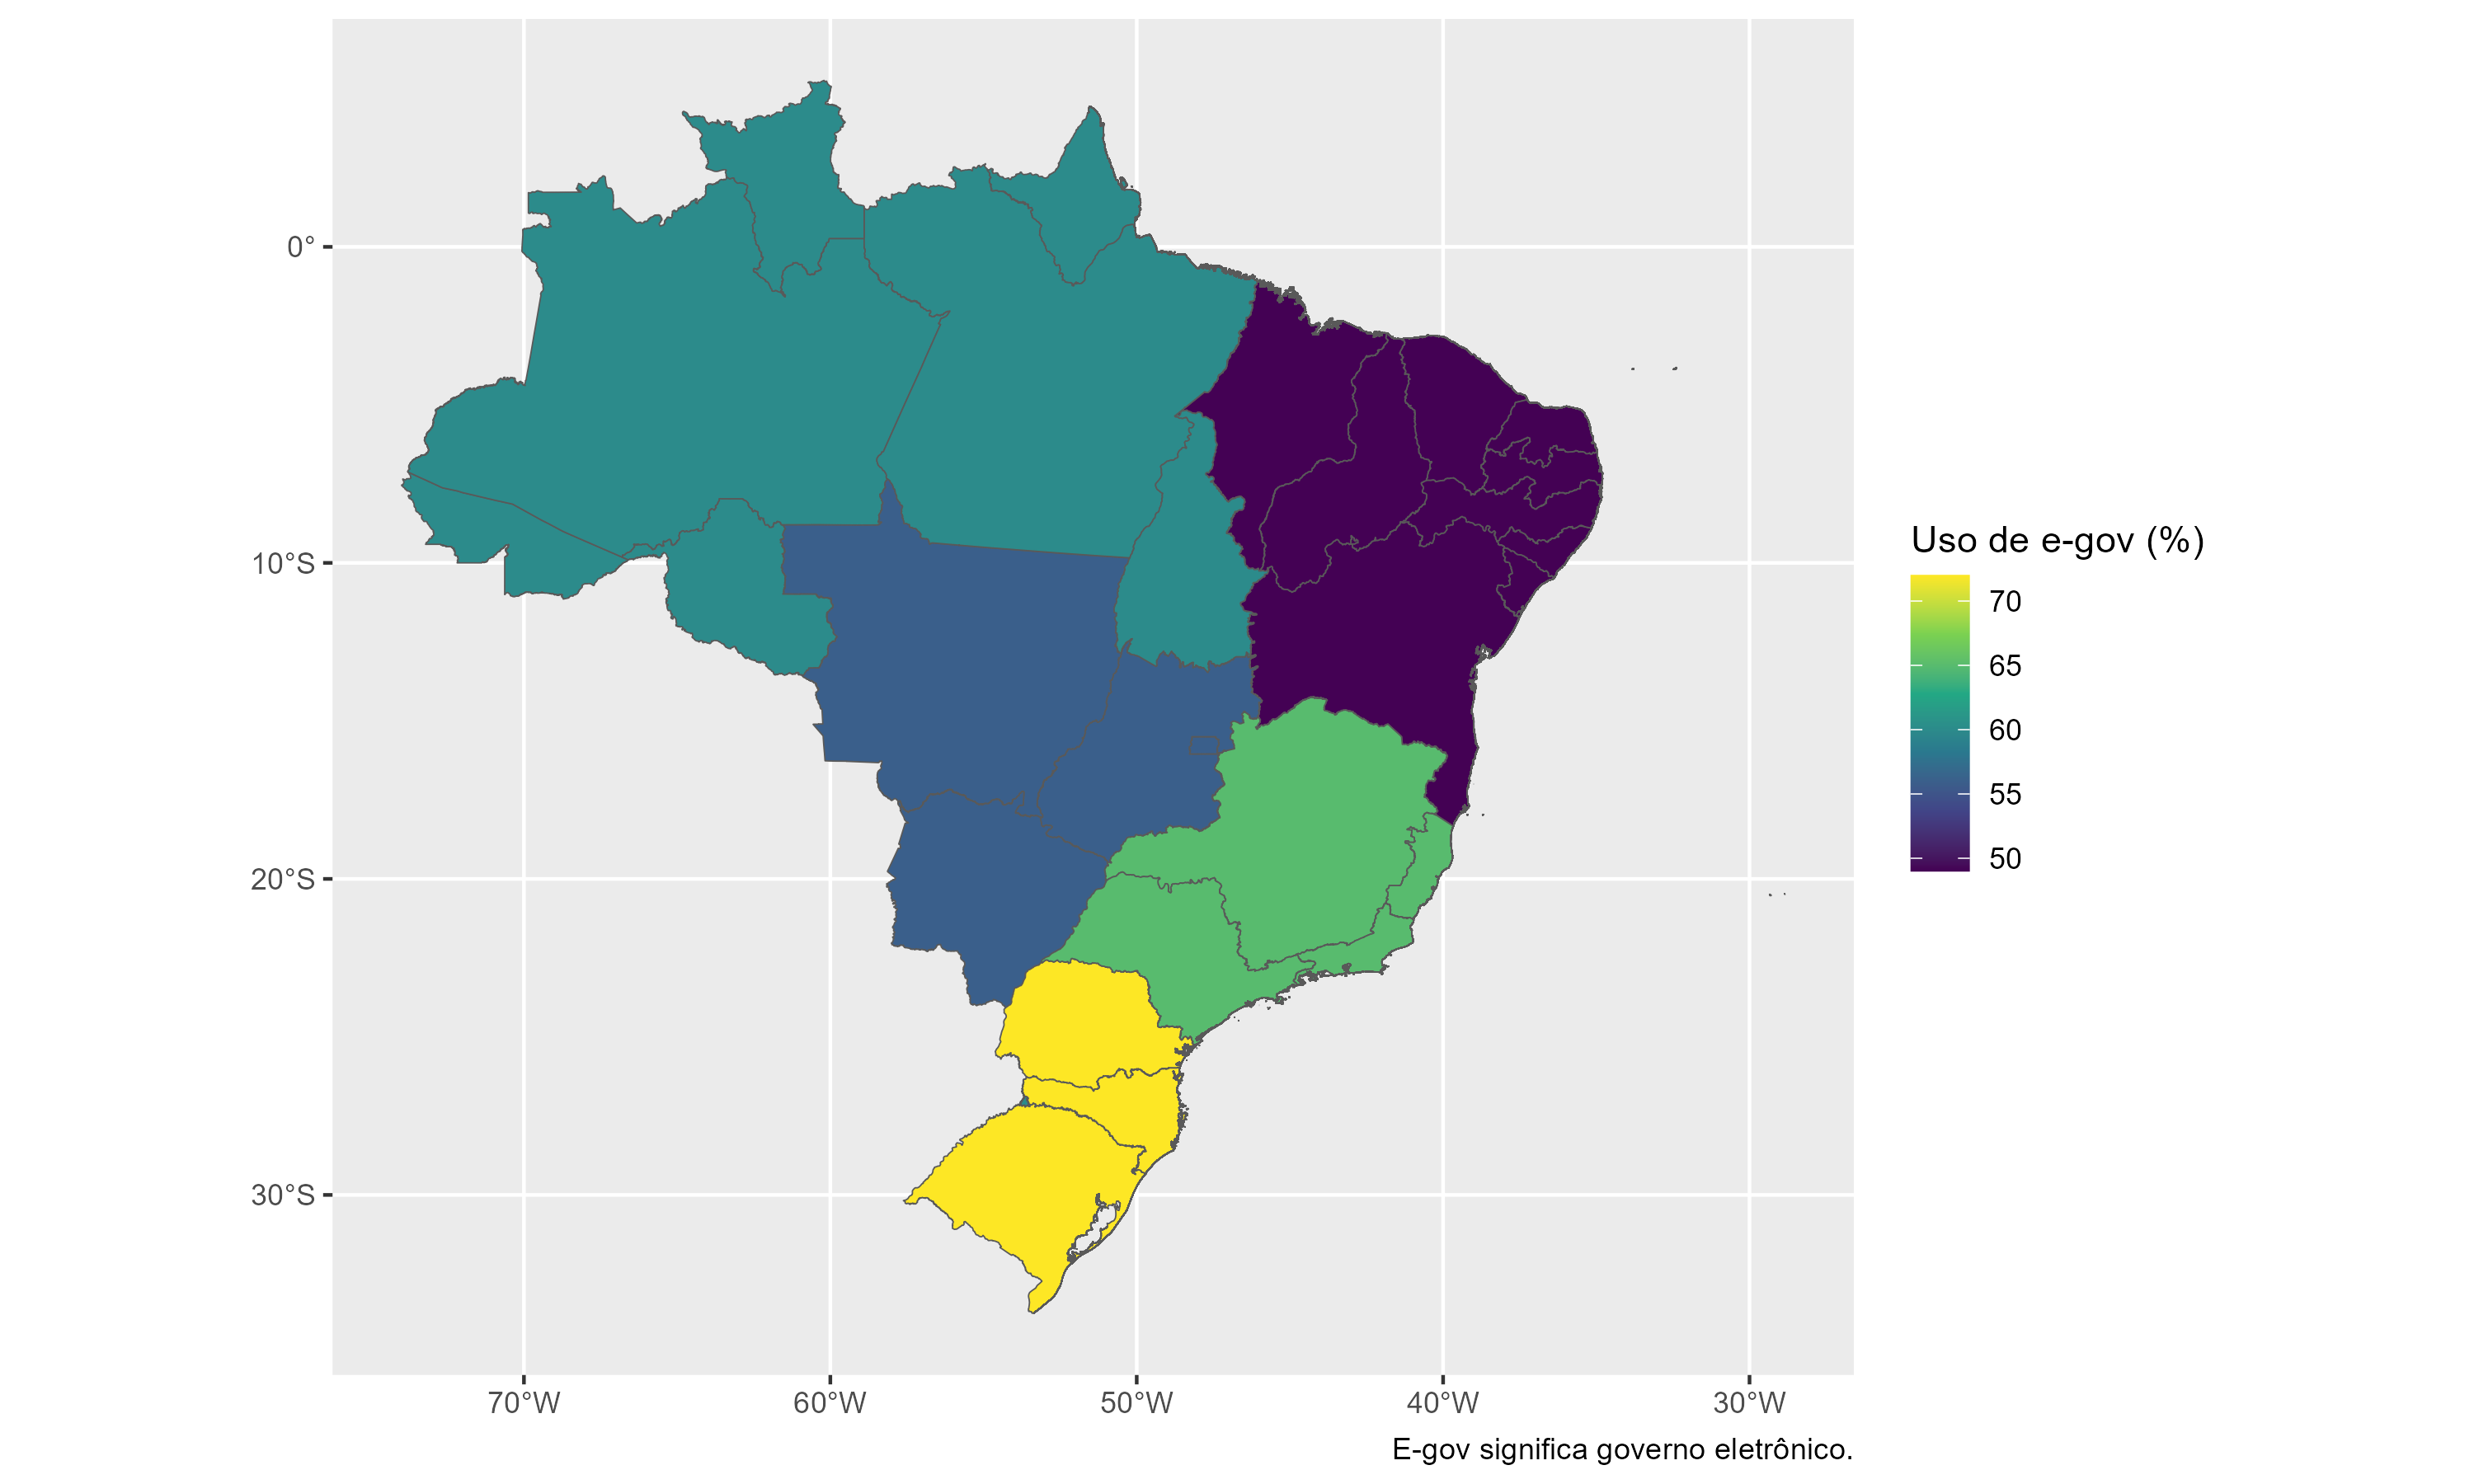
\includegraphics[width=1\linewidth]{figuras/mapa_coropleto_tic_domicilio_g1}
	\label{fig:mapa_coropleto_tic_domicilio_g1}
	\footnotesize{Fonte: \cite{tic_domicilios_2024_g1}}
\end{figure}

A figura \ref{fig:mapa_coropleto_tic_domicilio_g1} representa os resultados do indicador \href{https://cetic.br/pt/tics/domicilios/2024/individuos/G1/}{G1}. As regiões Sul e Sudeste são a regiões que mais usam ferramentas de governo eletrônico, seguidas das regiões Centro-Oeste e Norte. Por último, está o Nordeste. Serão elaborados mapas coropléticos dos indicadores \href{https://cetic.br/pt/tics/domicilios/2024/individuos/G2/}{G2} e \href{https://cetic.br/pt/tics/domicilios/2024/individuos/G3/}{G3}, respectivamente. Os códigos presentes nas tabelas \ref{tab:tic_domicilios_2024_g2} e \ref{tab:tic_domicilios_2024_g3} foram criados pelo auto para facilitar a identificação.

O indicador G2 tem os seguintes critérios:

\begin{longtable}{@{}p{0.18\textwidth} p{0.78\textwidth}@{}}
\caption{Critérios do indicador G2}
\label{tab:tic_domicilios_2024_g2} \\
\toprule
\textbf{Código} & \textbf{Critérios} \\
\midrule
\endfirsthead
\multicolumn{2}{@{}l@{}}{\textbf{Tabela \thetable{} -- continuação da página anterior}} \\
\toprule
\textbf{Código} & \textbf{Critérios} \\
\midrule
\endhead 
\midrule
\multicolumn{2}{r@{}}{\textit{Continua na próxima página}} \\
\endfoot
\bottomrule
\multicolumn{2}{r@{}}{\footnotesize{Fonte: baseado em \cite{tic_domicilios_2024_g2}}} \\
\endlastfoot
G2-A & \RaggedRight Documentos pessoais, como RG, CPF, passaporte ou carteira de trabalho \\
\midrule
G2-B & \RaggedRight Saúde pública, como agendamento de consultas, remédios ou outros serviços do sistema público de saúde \\
\midrule
G2-C & \RaggedRight Educação pública, como Enem, Prouni, matrículas em escolas ou universidades públicas \\
\midrule
G2-D & \RaggedRight Direito do trabalhador ou previdência social, como INSS, FGTS, seguro-desemprego, auxílio-doença ou aposentadoria \\
\midrule
G2-E & \RaggedRight Impostos e taxas governamentais, como declaração de imposto de renda, IPVA ou IPTU \\
\midrule
G2-F & \RaggedRight Polícia e segurança, como boletim de ocorrência, antecedentes criminais ou denúncias \\
\midrule
G2-G & \RaggedRight Transporte público ou outros serviços urbanos, como limpeza e conservação de vias, iluminação \\
\end{longtable}

Como foi demonstrado pela tabela \ref{tab:tic_domicilios_2024_g2}, o indicador G2 tem 7 critérios. Cada critério será representado por um mapa coroplético das regiões do Brasil representados nas figuras \ref{fig:mapa_coropleto_tic_domicilio_g2_A_B}, \ref{fig:mapa_coropleto_tic_domicilio_g2_C_D}, \ref{fig:mapa_coropleto_tic_domicilio_g2_E_F} e \ref{fig:mapa_coropleto_tic_domicilio_g2_G}.

\begin{figure}[H]
	\centering
	\caption{Indicadores G2: A e B}
	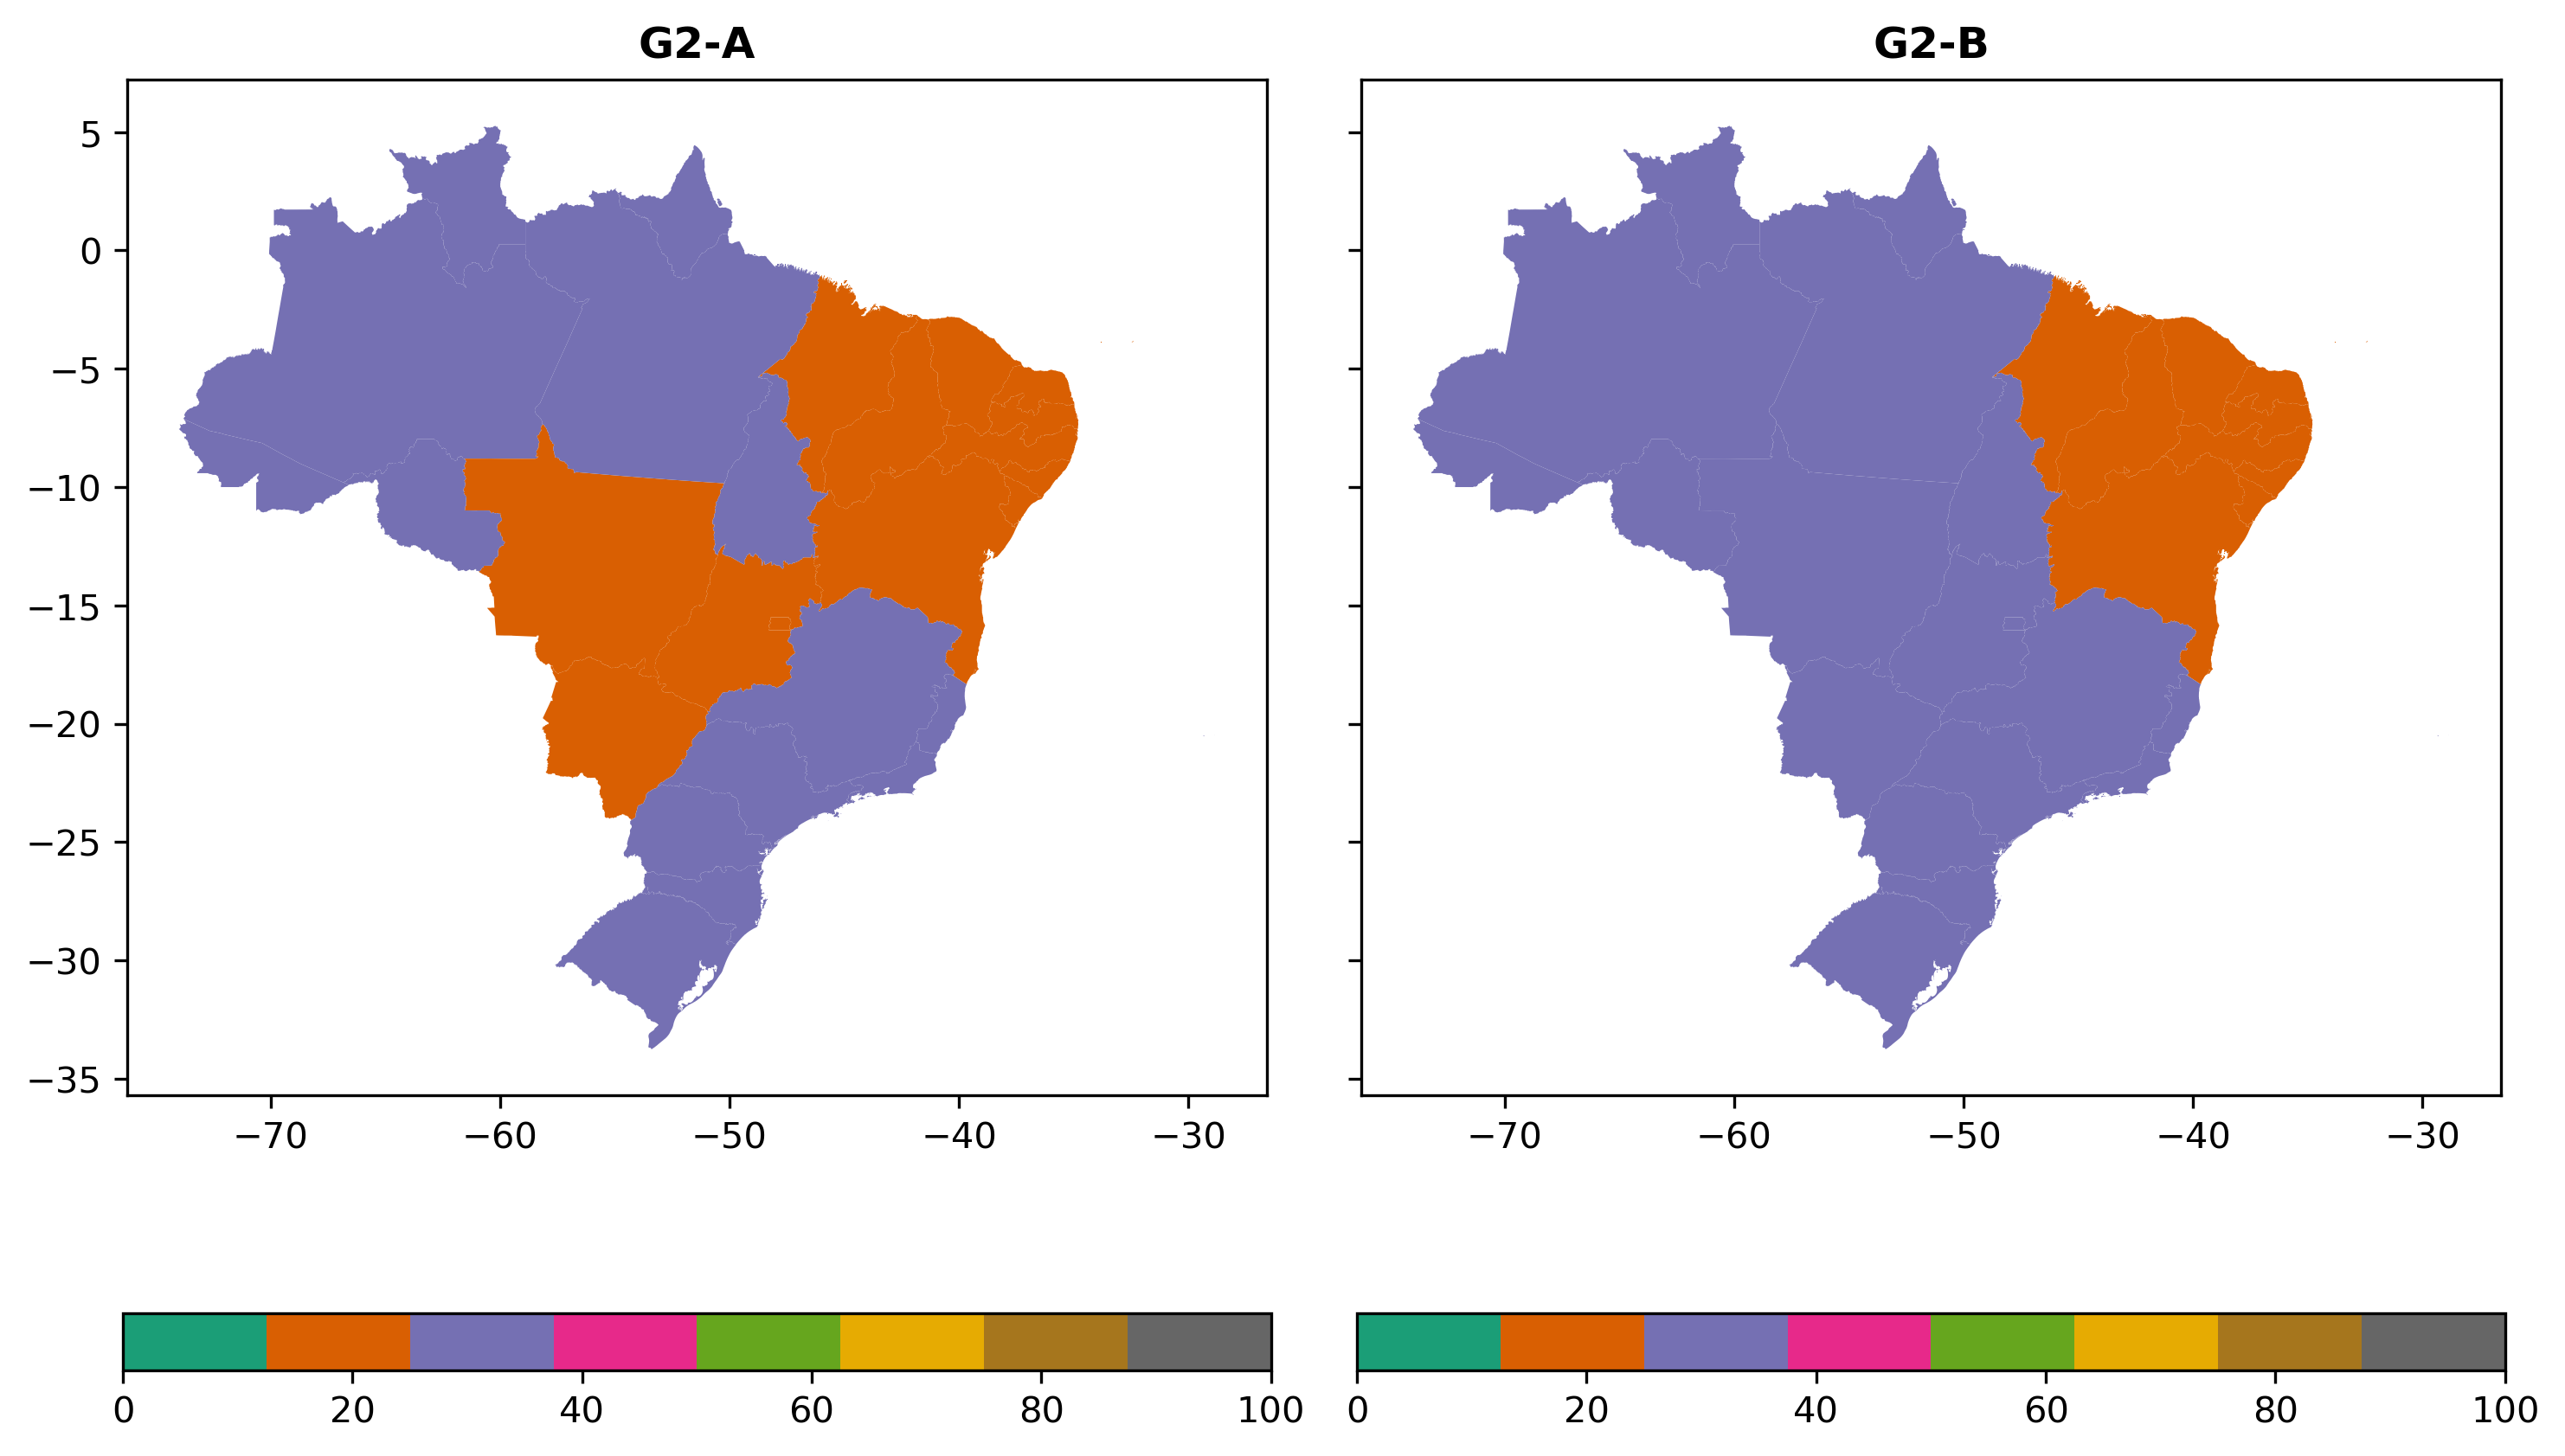
\includegraphics[width=1\linewidth]{figuras/mapa_coropleto_tic_domicilio_g2_A_B.png}
	\label{fig:mapa_coropleto_tic_domicilio_g2_A_B}
	\footnotesize{Fonte: \cite{tic_domicilios_2024_g2}}
\end{figure}

\begin{figure}[H]
	\centering
	\caption{Indicadores G2: C e D}
	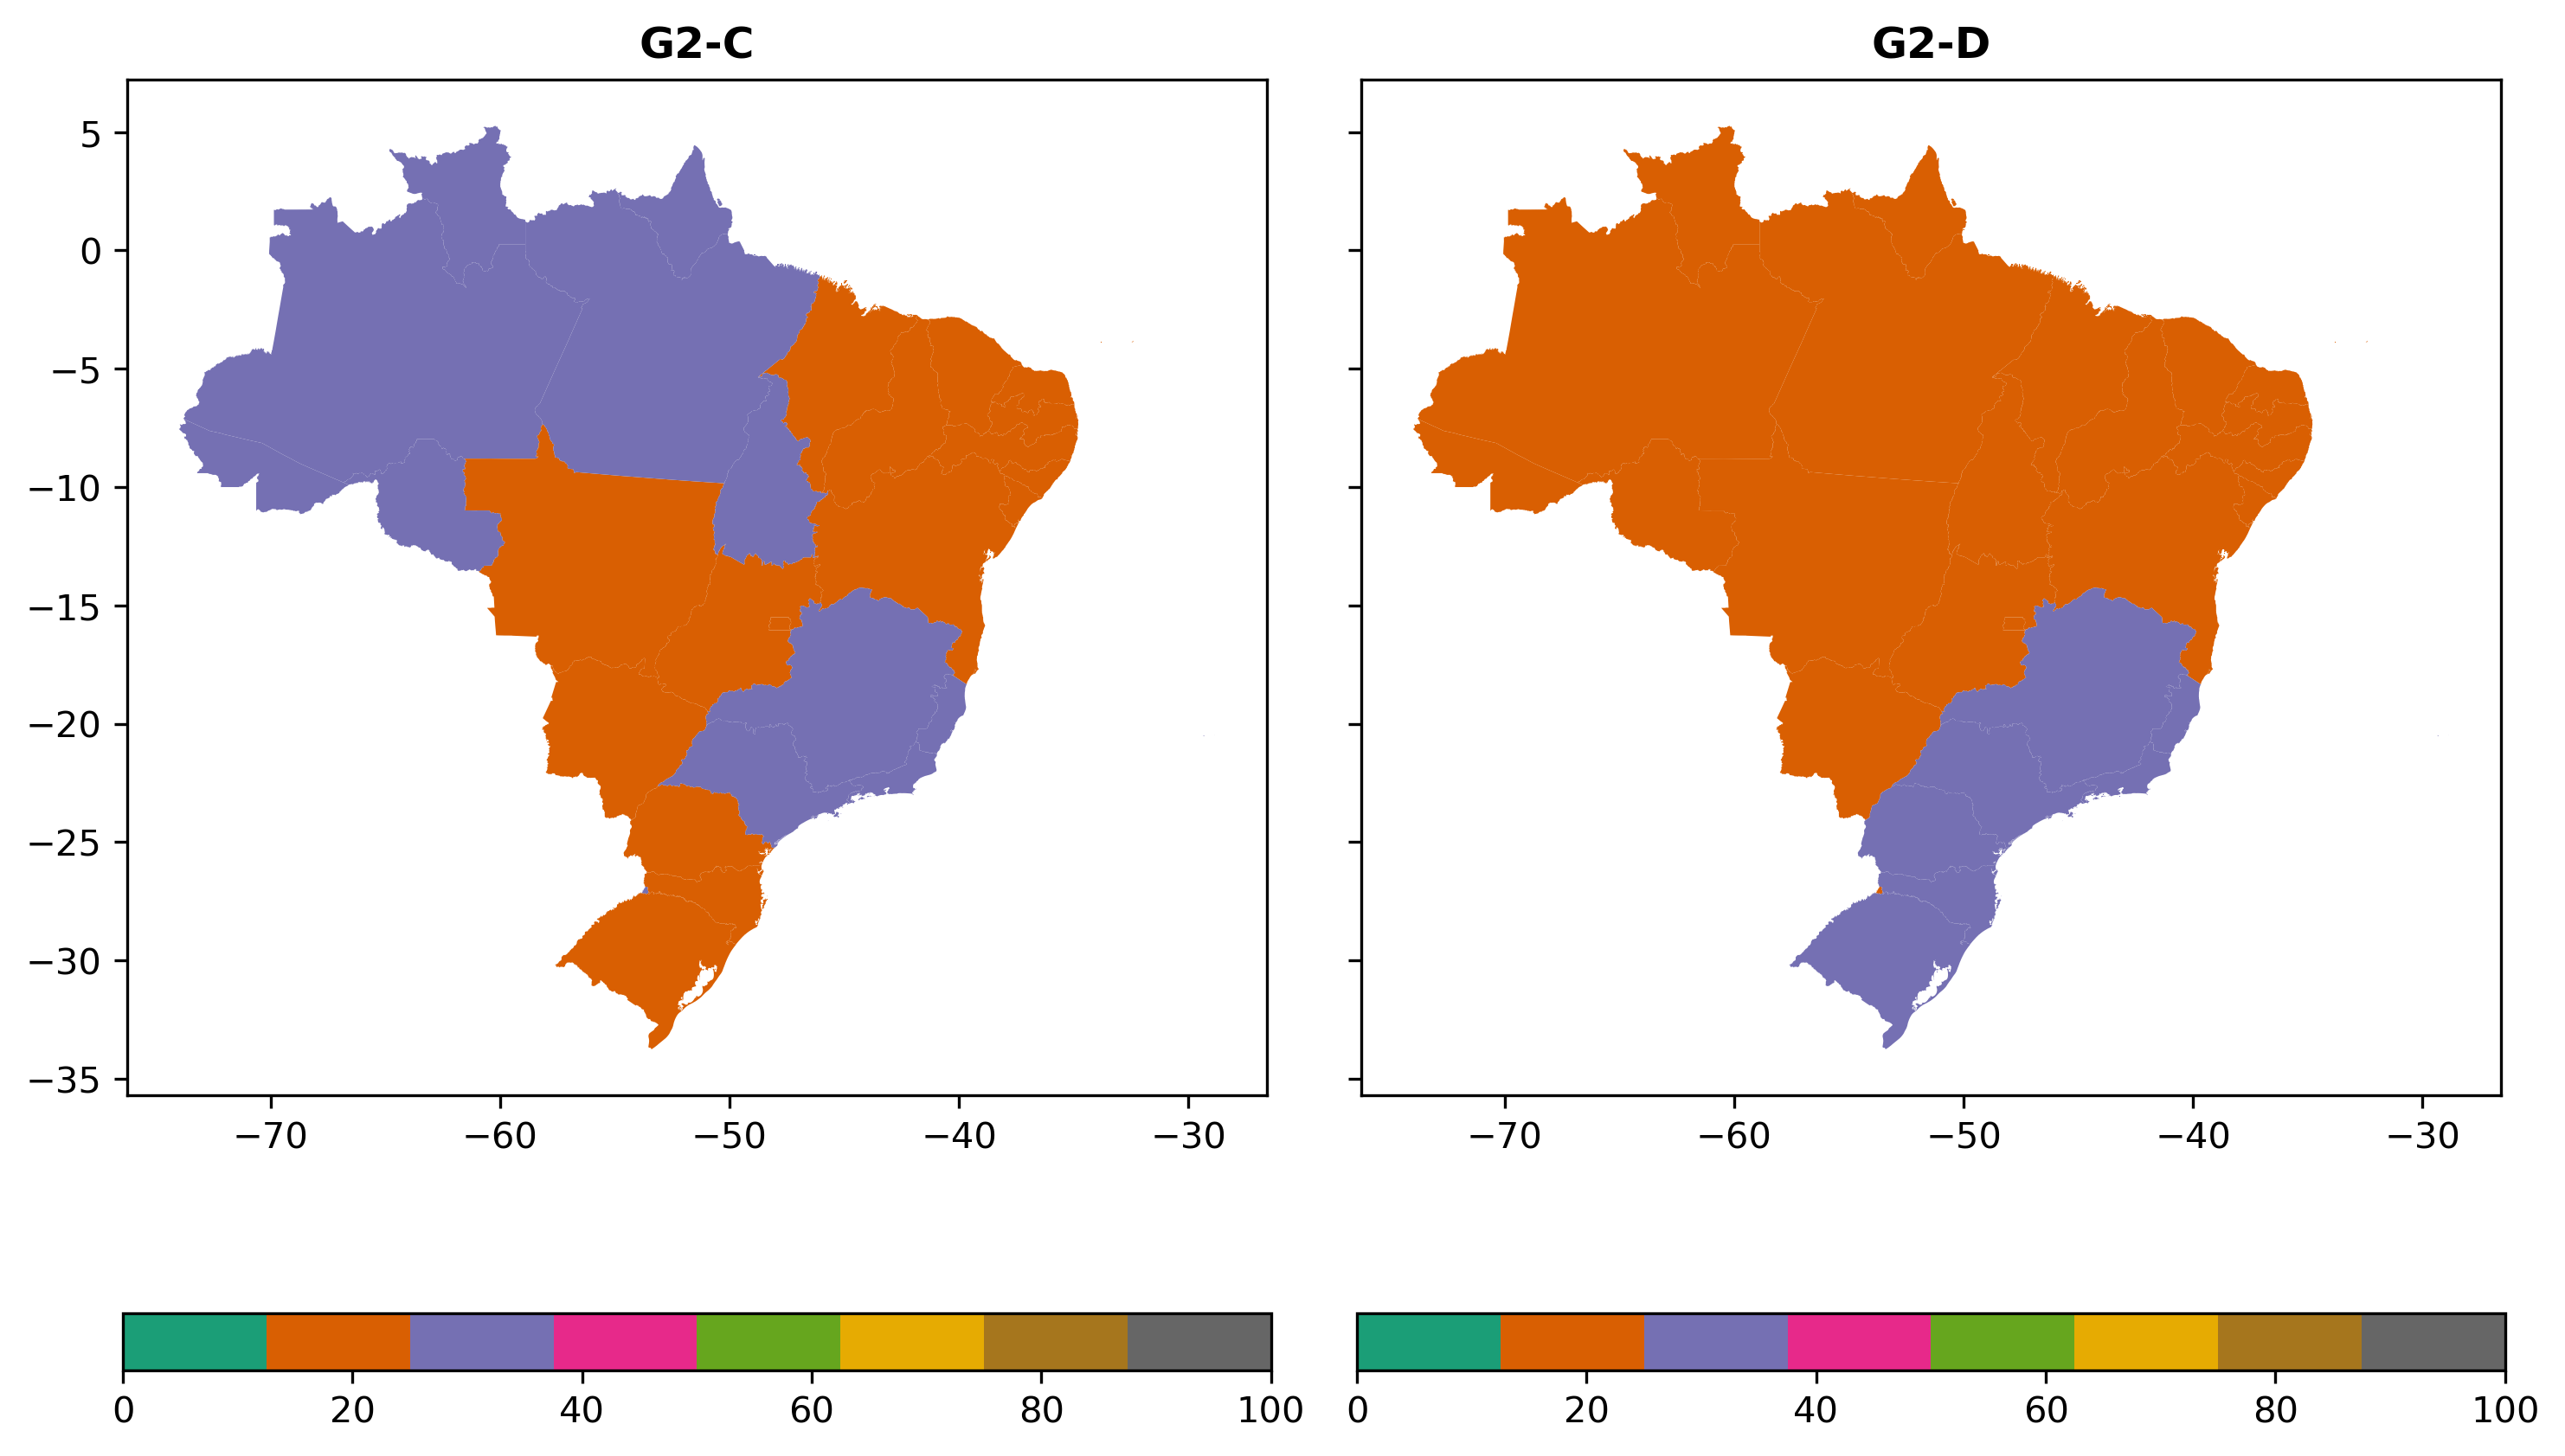
\includegraphics[width=1\linewidth]{figuras/mapa_coropleto_tic_domicilio_g2_C_D.png}
	\label{fig:mapa_coropleto_tic_domicilio_g2_C_D}
	\footnotesize{Fonte: \cite{tic_domicilios_2024_g2}}
\end{figure}

\begin{figure}[H]
	\centering
	\caption{Indicadores G2: E e F}
	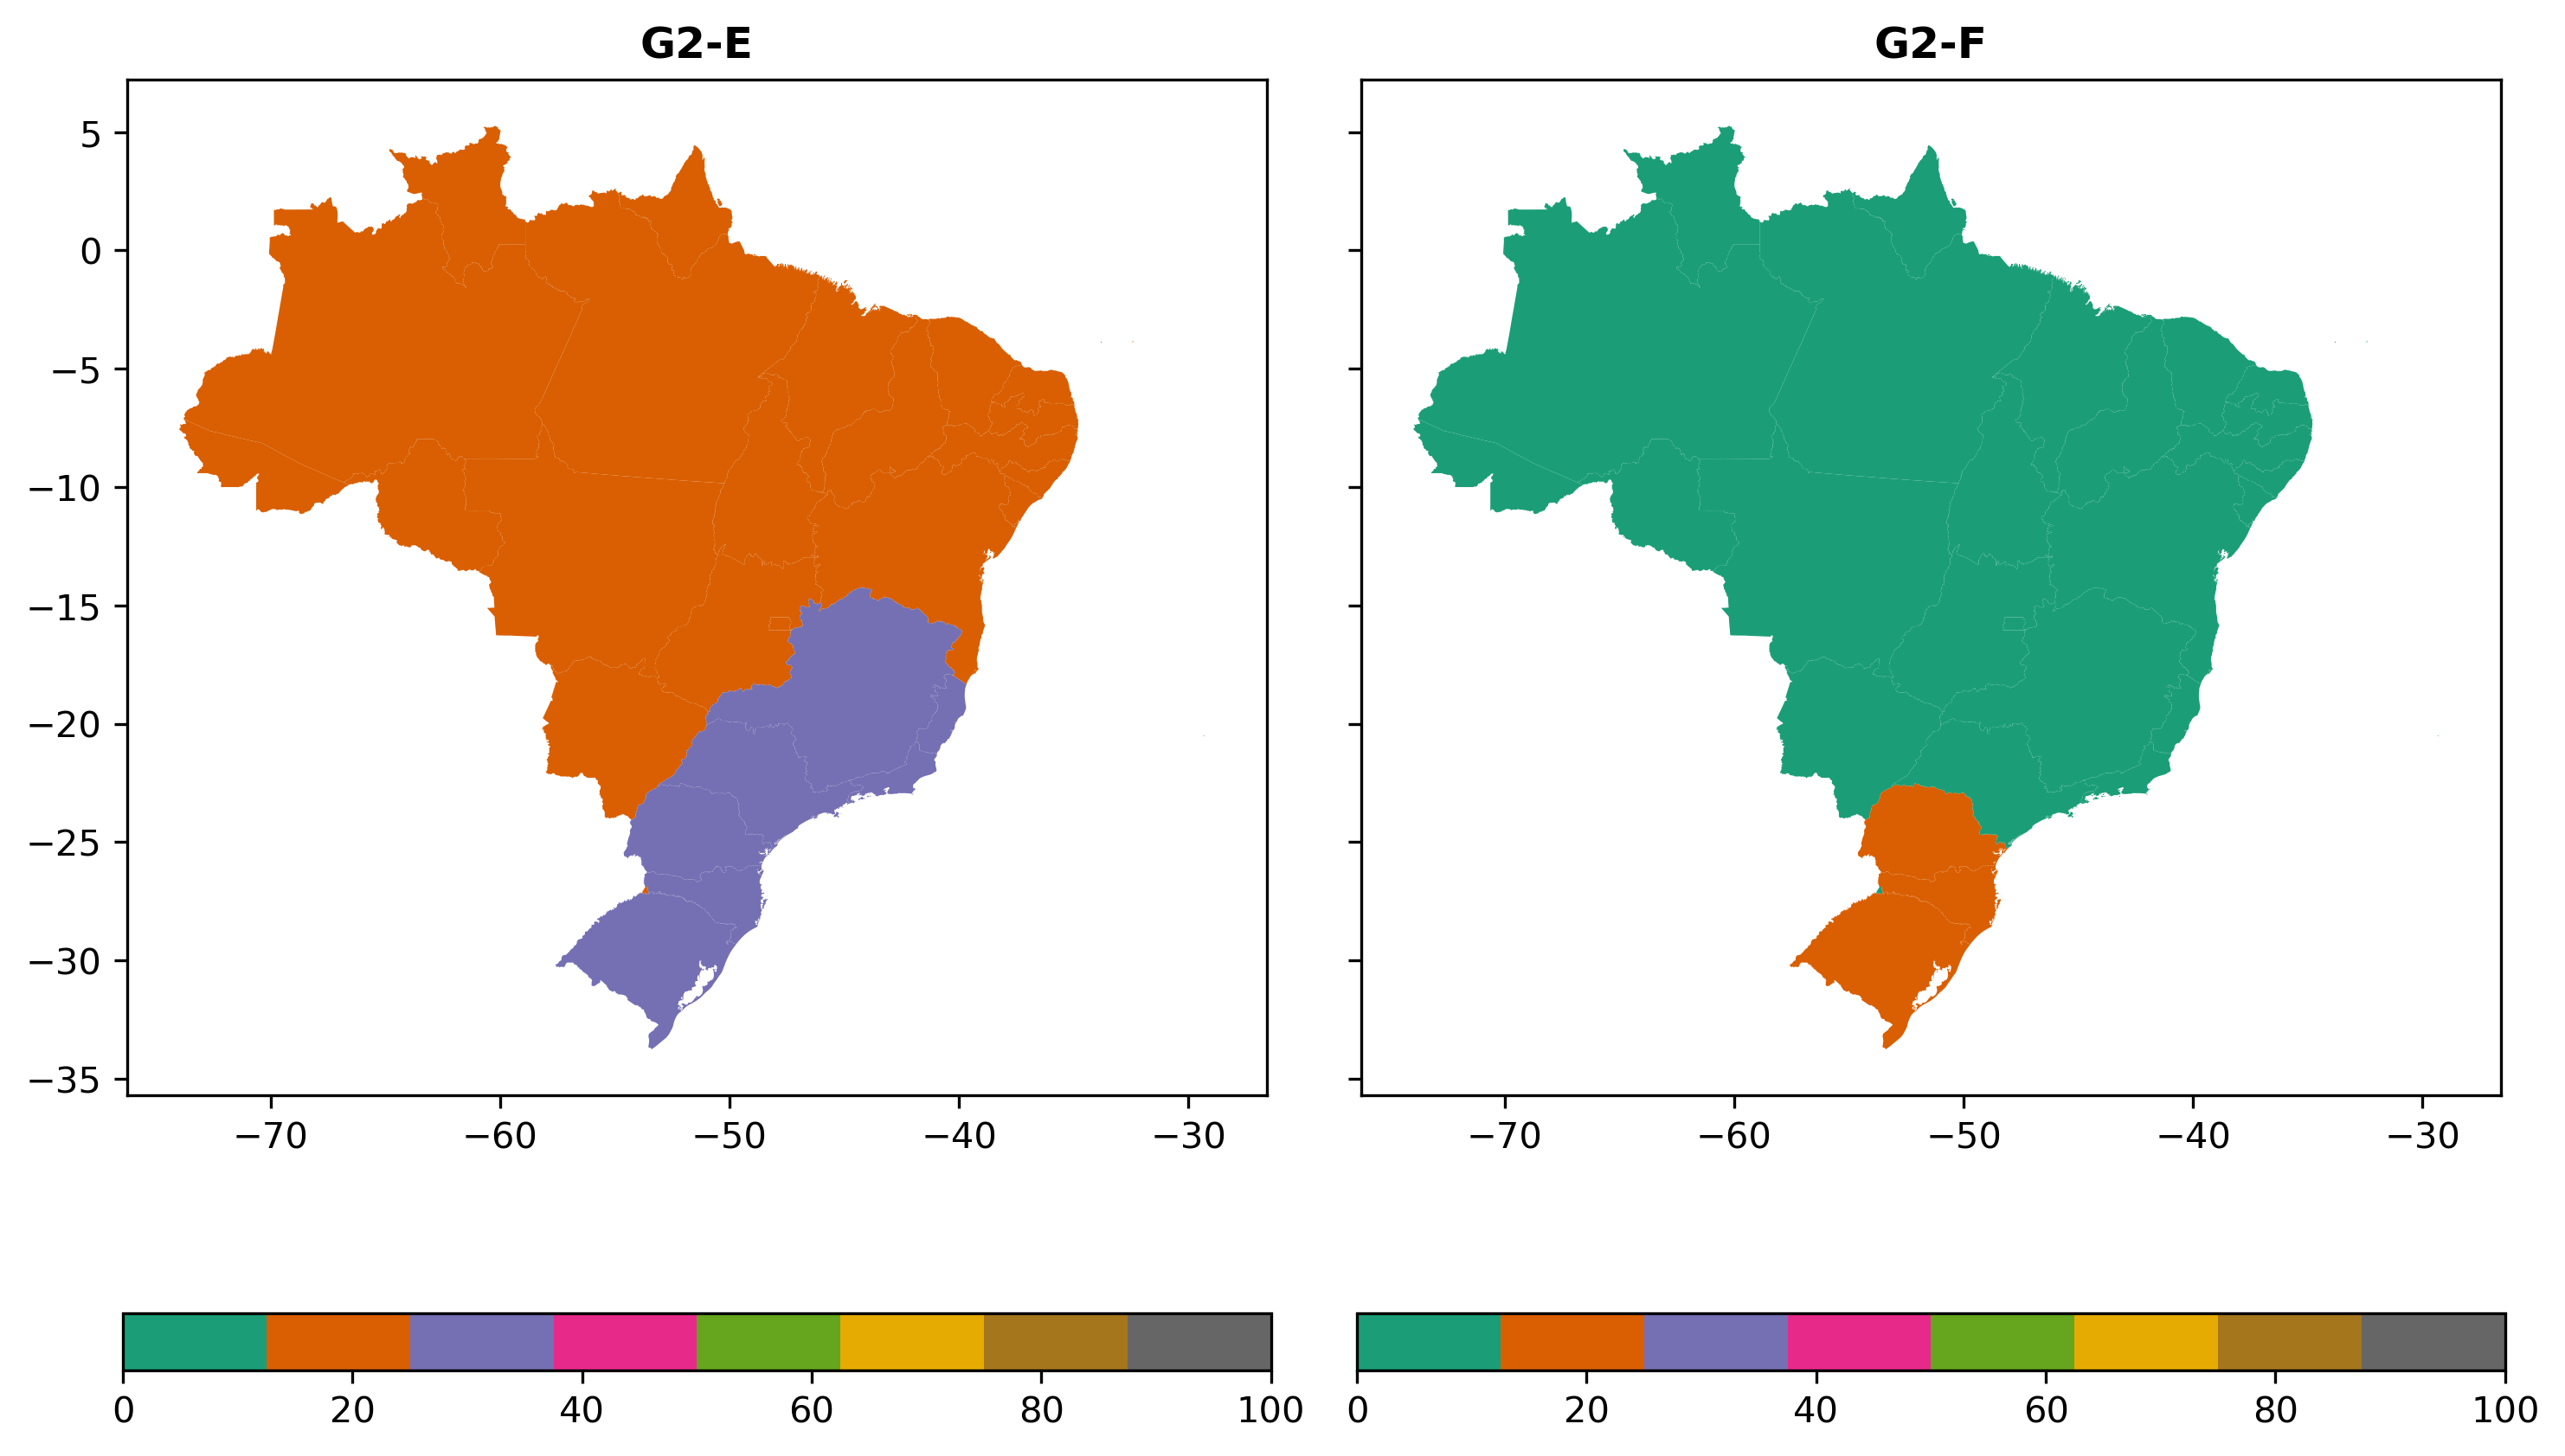
\includegraphics[width=1\linewidth]{figuras/mapa_coropleto_tic_domicilio_g2_E_F.png}
	\label{fig:mapa_coropleto_tic_domicilio_g2_E_F}
	\footnotesize{Fonte: \cite{tic_domicilios_2024_g2}}
\end{figure}

\begin{figure}[H]
	\centering
	\caption{Indicadores G2: G}
	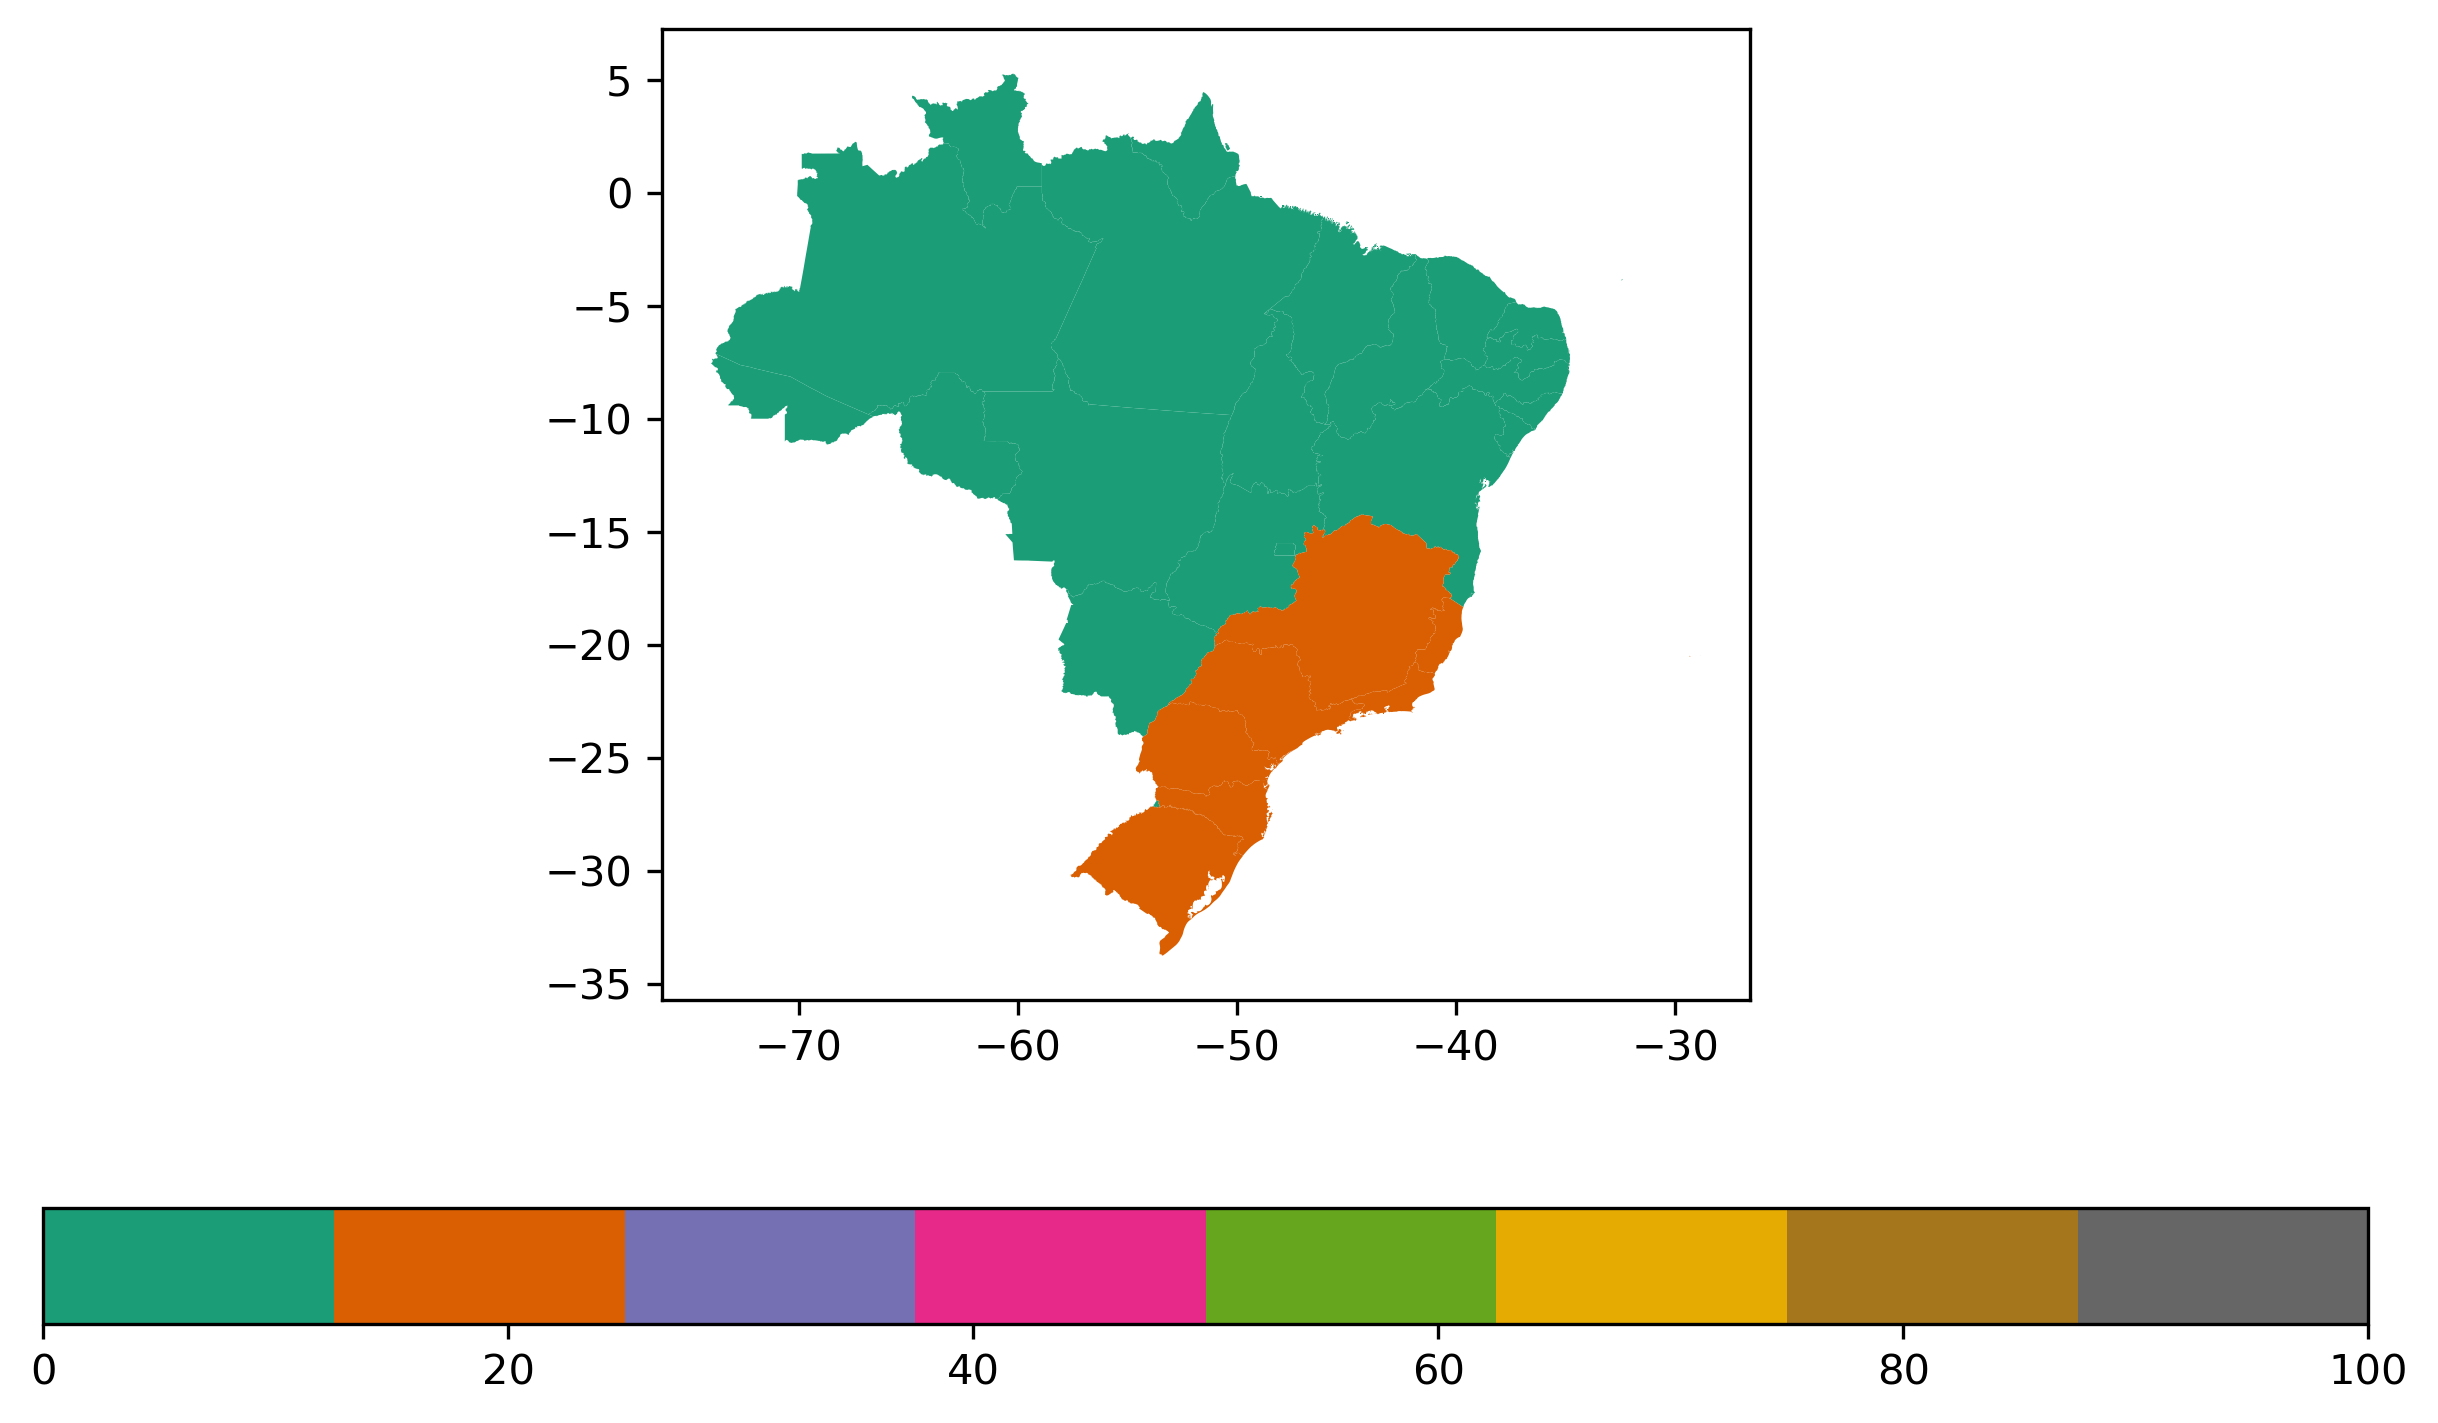
\includegraphics[width=1\linewidth]{figuras/mapa_coropleto_tic_domicilio_g2_G.png}
	\label{fig:mapa_coropleto_tic_domicilio_g2_G}
	\footnotesize{Fonte: \cite{tic_domicilios_2024_g2}}
\end{figure}